\section{Problem (7)}
	The figure shows two blocks connected by a cord (of negligible mass) that passes over a frictionless pulley (also of negligible mass). The arrangement is known as Atwood's machine. Block $1$ has mass $m_{1} = 0.89 \ kg$; block $2$ has mass $m_{2} = 1.44 \ kg$. What is the tension in the cord? Assume a $y$ axis has its positive direction upward.

	\begin{figure}[H]
		\begin{center}
			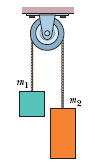
\includegraphics[scale=1]{hw5_problem7}
			\caption{Illustration of Problem 7}
			\label{fig:hw5_problem7}
		\end{center}
	\end{figure}

	\textbf{R:} \newline

	\begin{figure}[H]
		\begin{center}
			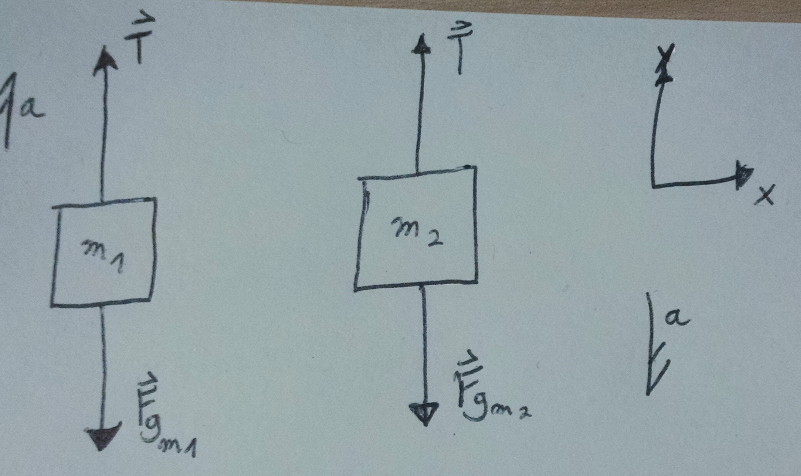
\includegraphics[scale=0.5]{hw5_problem7_fbd}
			\caption{Free-Body Diagram (Problem 7)}
			\label{fig:hw5_problem7_fbd}
		\end{center}
	\end{figure}

	For this problem, we can assume:
	\begin{itemize}
		\item{The tensions in both blocks are equals}
		\item{The aceleration in both blocks have the same magnitude}
	\end{itemize}

	Newton's $2^{nd}$ Law on Block $1$:
	\begin{align}
		\sum F_{y} = \ &m_{1}a_{y}& \notag \\
		T - F_{g_{y_{m_{1}}}} = \ &(0.89 \ kg)a& \notag \\
		T = \ &(0.89 \ kg)a + (0.89 \ kg)\left(9.8 \ m/s^{2}\right)& \notag \\
		T = \ &(0.89 \ kg)a + (8.72 \ N)& \notag
	\end{align}

	Newton's $2^{nd}$ Law on Block $2$:
	\begin{align}
		\sum F_{y} = \ &m_{2}a_{y}& \notag \\
		T - F_{g_{y_{m_{2}}}} = \ &(1.44 \ kg)(-a)& \notag \\
		T = \ &-(1.44 \ kg)a + (1.44 \ kg)\left(9.8 \ m/s^{2}\right)& \notag \\
		T = \ &-(1.44 \ kg)a + (14.112 \ N)& \notag
	\end{align}

	\begin{align}
		(0.89 \ kg)a + (8.72 \ N) = \ &-(1.44 \ kg)a + (14.112 \ N)& \notag \\
		(0.89 \ kg)a + (1.44 \ kg)a = \ & (14.112 \ N) - (8.72 \ N)& \notag \\
		(2.33 \ kg)a = \ & 5.392 \ N& \notag \\
		a = \ & \frac{5.392 \ N}{2.33 \ kg} = 2.314 \ m/s^{2}& \notag \\
		T = \ &(0.89 \ kg)(2.314 \ m/s^{2}) + (8.72 \ N)& \notag \\
		= \ &(2.06 \ N) + (8.72 \ N)& \notag \\
		= \ &10.78 \ N&
	\end{align}
